\documentclass{article}

\usepackage{arxiv}

\usepackage[utf8]{inputenc}
\usepackage[T1]{fontenc}
\usepackage{textcomp}
\usepackage{hyperref}
\usepackage{url}
\usepackage{booktabs}
\usepackage{amsfonts}
\usepackage{amssymb}
\usepackage{amsmath}
\usepackage{nicefrac}
\usepackage{microtype}
\usepackage{graphicx}
\usepackage[numbers]{natbib}
\usepackage{doi}
\usepackage{xcolor}

%% Unicode handlers (pdflatex)
\DeclareUnicodeCharacter{03B7}{$\eta$}
\DeclareUnicodeCharacter{2264}{$\leq$}
\DeclareUnicodeCharacter{2212}{$-$}
\DeclareUnicodeCharacter{2192}{$\rightarrow$}

\title{The Industrial Floor on the Cost of Fusion Electricity and the
Role of Direct Energy Conversion}

\author{%
        Tal Rubin\thanks{\texttt{tal.rubin@astera.org}} \\
        Astera Institute \\
        \And
        Damien Scott \\
        Astera Institute
}

\renewcommand{\shorttitle}{Floor and DEC}

\hypersetup{
pdftitle={The Industrial Floor on the Cost of Fusion Electricity and the Role of Direct Energy Conversion},
pdfauthor={Tal Rubin, Damien Scott},
pdfkeywords={fusion energy, LCOE, balance of plant, direct energy conversion, aneutronic fusion, p-B11, D-He3},
}

\begin{document}
\maketitle

\begin{abstract}
The levelized cost of electricity (LCOE) of a fusion power plant is
analyzed under two complementary lenses. An industrial \emph{cost
floor} is first computed by setting the fusion core to zero capital
cost, isolating the irreducible contribution of buildings,
balance-of-plant equipment, operations and maintenance, and financing.
Within the open-source \texttt{1costingfe} model, this floor is
governed primarily by fuel choice rather than by plant design. A
deuterium-tritium plant exhibits a baseline floor of \$29/MWh at
1\,GWe, falling to \$9.6/MWh only at 5\,GWe under aggressive
financial and operational assumptions; a proton-boron-11 plant
attains \$18/MWh at baseline and \$5.3/MWh at the same aggressive
limit, leaving meaningful budget for the costed core. Two
charged-particle direct energy conversion (DEC) architectures are
then evaluated against thermal-cycle baselines: a venetian-blind
collector applicable to linear devices and an inductive recovery
scheme applicable to compressed plasmoids. For p-B11, bremsstrahlung
carries 83\% of the fusion power and constrains DEC to capturing only
the charged-particle margin, producing no measurable reduction in the
balance-of-plant floor. For D-He3, an inductive scheme reduces the
required fusion power and the helium-3 burn rate but substitutes a
pulsed-power chain whose cost exceeds that of a steam turbine of
equivalent capacity. DEC therefore exerts leverage on the costed core
and on the fuel bill, not on the industrial floor.
\end{abstract}

\keywords{fusion energy \and LCOE \and balance of plant \and direct
energy conversion \and aneutronic fusion}

\section{Introduction}
\label{sec:intro}

Published estimates for the levelized cost of electricity (LCOE)
from commercial fusion power plants span more than an order of
magnitude. Optimistic n-th-of-a-kind advanced tokamaks have been
projected at \$47/MWh \citep{Najmabadi2006}; first-generation
EU-DEMO scenarios reach \$160/MWh and above \citep{Entler2018}; most
serious estimates fall between \$50 and \$130/MWh
\citep{SheffieldMilora2016, Lindley2023}. A recent compilation of
first-of-a-kind capital expenditure estimates reports an
approximately thirty-fold spread, from \$1{,}400 to \$43{,}000 per
kilowatt installed \citep{Tang2026}. The variability reflects genuine
disagreement about the cost of the fusion core (magnets, blanket,
heating systems, vacuum vessel, structure), which has no current
deployed analog at utility scale.

This paper examines the cost target of one cent per kilowatt-hour
(\$10/MWh) by separating the question into two components.
Section~\ref{sec:floor} characterizes the cost floor that remains
when the fusion core is assumed to cost nothing, isolating the
contribution of buildings, balance-of-plant equipment, indirect
costs, owner's costs, supplementary costs, financing charges, and
operations and maintenance, all of which exist regardless of the
specific core technology. Section~\ref{sec:dec} examines the choice
of energy conversion architecture: a thermal cycle is the default,
but for fuels in which the energy emerges predominantly as charged
particles, direct energy conversion (DEC) provides an alternative
with a different cost structure. Two charged-particle DEC
architectures are evaluated: a venetian-blind collector and a pulsed
inductive scheme.

The cost analysis is performed using
\texttt{1costingfe}\footnote{\url{https://github.com/1cfe/1costingfe}},
an open-source techno-economic model whose methodology is documented
elsewhere. All numerical results can be reproduced with the companion
scripts in that repository.

\section{The Industrial Cost Floor with a Free Fusion Core}
\label{sec:floor}

The lower bound on fusion LCOE imposed by non-core plant elements is
characterized first. The fusion core is assigned zero capital cost,
zero on-site footprint, and zero contribution to staffing
requirements. The remaining plant must still convert the fusion
energy into electricity, contain whatever radiation hazards the fuel
imposes, and operate as a utility-scale generation asset. A
schematic of the constituent systems is shown in
Figure~\ref{fig:plant}.

\begin{figure}[htbp]
\centering
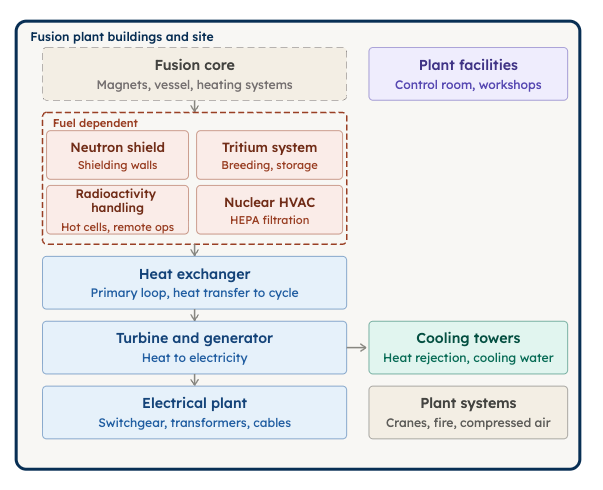
\includegraphics[width=0.7\linewidth]{figures/power_plant_schematic.png}
\caption{Schematic of a fusion power plant with thermal power
conversion. Building scope, balance-of-plant equipment (turbine
island, electrical plant, heat rejection), and staffing all retain
a fuel-dependent component. The fusion core (left of the heat
exchanger) is assigned zero capital cost in the floor analysis of
Section~\ref{sec:floor}.}
\label{fig:plant}
\end{figure}

\subsection{Thermal Balance of Plant}
\label{sec:bop}

Most fusion concepts assume a thermal cycle in which the fusion core
delivers heat to a working fluid that drives a turbine and
generator. The balance of plant (BOP) comprises the turbine and
generator, electrical plant equipment (switchgear, transformers,
grid connection), miscellaneous mechanical equipment (cranes,
compressed air, fire protection), and heat rejection (cooling towers
and circulating water). These are mature industrial systems with
well-characterized pricing and negligible learning rate.

For a 1\,GWe plant equipped with a supercritical CO\textsubscript{2}
Brayton cycle (the lowest-floor option among Rankine,
sCO\textsubscript{2}, and combined-cycle alternatives), the BOP
equipment subtotal is \$390M
(Table~\ref{tab:bop}). Equipment unit costs are derived from the
NETL Cost and Performance Baseline for Fossil Energy Plants
\citep{NETL2022} and the ARIES cost account documentation
\citep{Waganer2013}, escalated to 2024 dollars. For aneutronic fuel
cycles, the share of fusion energy entering the thermal cycle is
reduced by the fraction routed through DEC; because bremsstrahlung
deposits the majority of the fusion energy on the first wall
(Section~\ref{sec:dec}), the thermal cycle remains the primary power
conversion pathway and the turbine downsizing is modest, dropping
the BOP subtotal to \$374M.

\begin{table}[htbp]
\caption{Thermal balance-of-plant equipment costs for a 1\,GWe D-T
fusion plant with sCO\textsubscript{2} Brayton cycle (2024 USD).}
\label{tab:bop}
\centering
\begin{tabular}{lrl}
\toprule
Component & Cost & Description \\
\midrule
Turbine and generator & \$180M & sCO\textsubscript{2}
turbomachinery, comparable to gas plant hardware \\
Electrical plant & \$98M & Switchgear, transformers, grid
connection \\
Miscellaneous equipment & \$60M & Cranes, compressed air, fire
protection \\
Heat rejection & \$55M & Cooling towers, circulating water \\
\midrule
\textbf{Subtotal} & \textbf{\$390M} & \\
\bottomrule
\end{tabular}
\end{table}

\subsection{Buildings and Site Structures}
\label{sec:buildings}

A fusion plant comprises 18 distinct buildings and
site structures: reactor building, turbine hall, heat-exchanger
building, cryogenics facility, power-supply building, control room,
maintenance shops, and others. Roughly half of these (turbine hall,
cryogenics facility, switchgear, assembly hall) are common to all
fuel cycles. The other half varies with the radiation and tritium
hazards of the chosen fuel.

A D-T plant requires biological shielding within the reactor
building, a hot cell for remote handling of activated components
(\$90M alone), tritium containment barriers, and nuclear-grade HVAC
with HEPA filtration. A D-He3 plant retains some radiation shielding
and tritium monitoring (owing to D-D side reactions), but at reduced
scope. An aneutronic p-B11 plant requires none of the above: the
reactor building is a standard heavy industrial crane hall, no hot
cell is required, and HVAC is conventional. Building costs at
1\,GWe consequently range from \$354M for p-B11 to \$570M for D-T
(Table~\ref{tab:fuels}).

\subsection{The D-T Floor}
\label{sec:dt}

Combining BOP, buildings, indirect costs (engineering and project
management, 20\% of directs), owner's costs,
supplementary costs (shipping, spares, insurance, decommissioning
provisions), and financing charges (interest during construction)
yields a total capital cost of \$1{,}700M for a 1\,GWe D-T plant
with a free fusion core. Operations and maintenance, dominated by
staffing of 78 full-time-equivalent employees (FTE) at
1\,GWe to cover health physics, tritium handling, radioactive waste
disposition, and hot cell operations, contributes \$18--40M per
year. Under standard financial assumptions (7\% weighted average
cost of capital, 85\% availability, 30-year lifetime, 6-year
construction), the LCOE floor is \$29/MWh, exceeding the one-cent
target by a factor of approximately 2.9.

For comparison, the fully costed D-T tokamak LCOE under the same
conditions is \$83/MWh; the fusion core accounts for approximately
two-thirds of this. The remaining third (the floor characterized
here) already exceeds the one-cent target, so no improvement to the
core can close a gap that lies outside it.

The parameters that lower the floor without reducing core cost are
plant scale (which spreads fixed costs over more megawatt-hours),
availability, weighted average cost of capital (WACC), construction
duration (which determines interest during construction), plant
lifetime, and staffing. Pushing each parameter toward favorable but
plausible values (Table~\ref{tab:dt-sweep}) reduces the D-T floor to
\$9.6/MWh only at the most aggressive combination: 5\,GWe net
output, 95\% availability, 2\% WACC, 50-year lifetime, and 3-year
construction. Even at this limit, the budget remaining for the
fusion core is \$0.4/MWh, equivalent to roughly \$40/kW of
overnight capital for the entire core, less than the cost of a
single large superconducting magnet. The D-T floor cannot be
lowered sufficiently to leave material budget for the costed core
within the parameter space considered.

\begin{table}[htbp]
\caption{D-T floor LCOE and overnight capital cost as a function of
plant scale and financial parameters, with a free fusion core.}
\label{tab:dt-sweep}
\centering
\begin{tabular}{lrrr}
\toprule
Scenario (D-T) & Floor (\$/MWh) & Overnight (\$/kW) & Core
budget (\$/MWh)\footnote{Core budget = \$10/MWh target minus floor;
negative values indicate the floor alone exceeds the one-cent
target.} \\
\midrule
Baseline: 1\,GWe, 85\%, 7\%, 30\,yr, 6\,yr & 29 & 1{,}720 & $-19$ \\
2\,GWe, 85\%, 7\%, 30\,yr, 6\,yr & 24 & 1{,}500 & $-14$ \\
2\,GWe, 95\%, 3\%, 50\,yr, 3\,yr & 14 & 1{,}210 & $-3.7$ \\
3\,GWe, 95\%, 3\%, 50\,yr, 3\,yr & 12 & 1{,}150 & $-2.0$ \\
5\,GWe, 95\%, 2\%, 50\,yr, 3\,yr & 9.6 & 1{,}090 & $+0.4$ \\
\bottomrule
\end{tabular}
\end{table}

For brevity, the combination of 2\,GWe, 95\% availability, 3\% WACC,
50-year lifetime, and 3-year construction is referred to below as
the \emph{aggressive scenario}.

The constraint is structural. D-T buildings cost \$570M because
neutrons and tritium impose shielding, hot cells, containment, and
nuclear-grade HVAC. D-T staffing approaches 78 FTE because those
hazards require health physics technicians, tritium processing and
accountability personnel, radioactive waste handlers, and hot cell
operators. These costs scale weakly with plant size and do not
disappear; they are consequences of the fuel choice rather than of
the plant design.

\subsection{Aneutronic Fuel Cycles}
\label{sec:aneutronic}

Different fuel choices yield different floors
(Table~\ref{tab:fuels}). Deuterium-helium-3 (D-He3) produces
approximately 6\% of its primary-reaction energy as neutrons via
D-D side reactions, requiring some shielding and modest tritium
monitoring; buildings amount to \$388M and the BOP-only floor at
1\,GWe is \$19/MWh. The D-He3 plant carries a separate burden:
at an optimistic helium-3 price of \$2M/kg, fuel contributes
\$74/MWh to LCOE \citep{Shea2010}; the DOE-allocated price of
approximately \$4.5M/kg doubles this. Helium-3 is not
produced at commercial scale, and breeding it would likely require
a separate D-D fusion source.

Proton-boron-11 (p-B11) is aneutronic: 99.8\% of the
primary-reaction energy emerges as charged alpha particles.
Buildings are constructed to conventional industrial standards,
yielding \$354M at 1\,GWe and a BOP-only floor of \$18/MWh.
Staffing requirements correspond to those of a conventional thermal
plant supplemented by fusion-specific roles (magnet technicians,
vacuum systems, plasma control), without radiation-specific
positions.

\begin{table}[htbp]
\caption{Building cost, BOP-only floor LCOE, and staffing as a
function of fuel cycle at 1\,GWe with a free fusion core.}
\label{tab:fuels}
\centering
\begin{tabular}{lrrr}
\toprule
Fuel & Buildings (1\,GWe) & BOP floor & Staffing \\
\midrule
D-T & \$570M & \$29/MWh & 78 FTE \\
D-He3 & \$388M & \$19/MWh & 39 FTE \\
p-B11 & \$354M & \$18/MWh & 36 FTE \\
\bottomrule
\end{tabular}
\end{table}

The \$220M building cost gap between D-T and p-B11 at 1\,GWe is
larger than most fusion-core cost-reduction scenarios in the
literature. The gap reflects the implications of handling neutrons
and tritium, not the difficulty of the underlying plasma physics.
The fuel choice establishes the floor before the fusion core enters
the calculation.

For p-B11 under the aggressive scenario, the floor falls to
\$7.6/MWh, leaving \$2.4/MWh for the fusion core (approximately
\$920/kW of overnight capital). This figure is comparable to the
overnight cost of a natural gas combined-cycle plant
(\$900--1{,}200/kW), with the difference that the fusion core
lacks the deployment scale and manufacturing maturity of
combined-cycle hardware. At 5\,GWe, 2\% WACC, 50-year life, and
3-year construction, the p-B11 floor falls to \$5.3/MWh.

Floor LCOE values across fuel cycles and scenario levels are
summarized in Figure~\ref{fig:lower-bound}.

\begin{figure}[htbp]
\centering
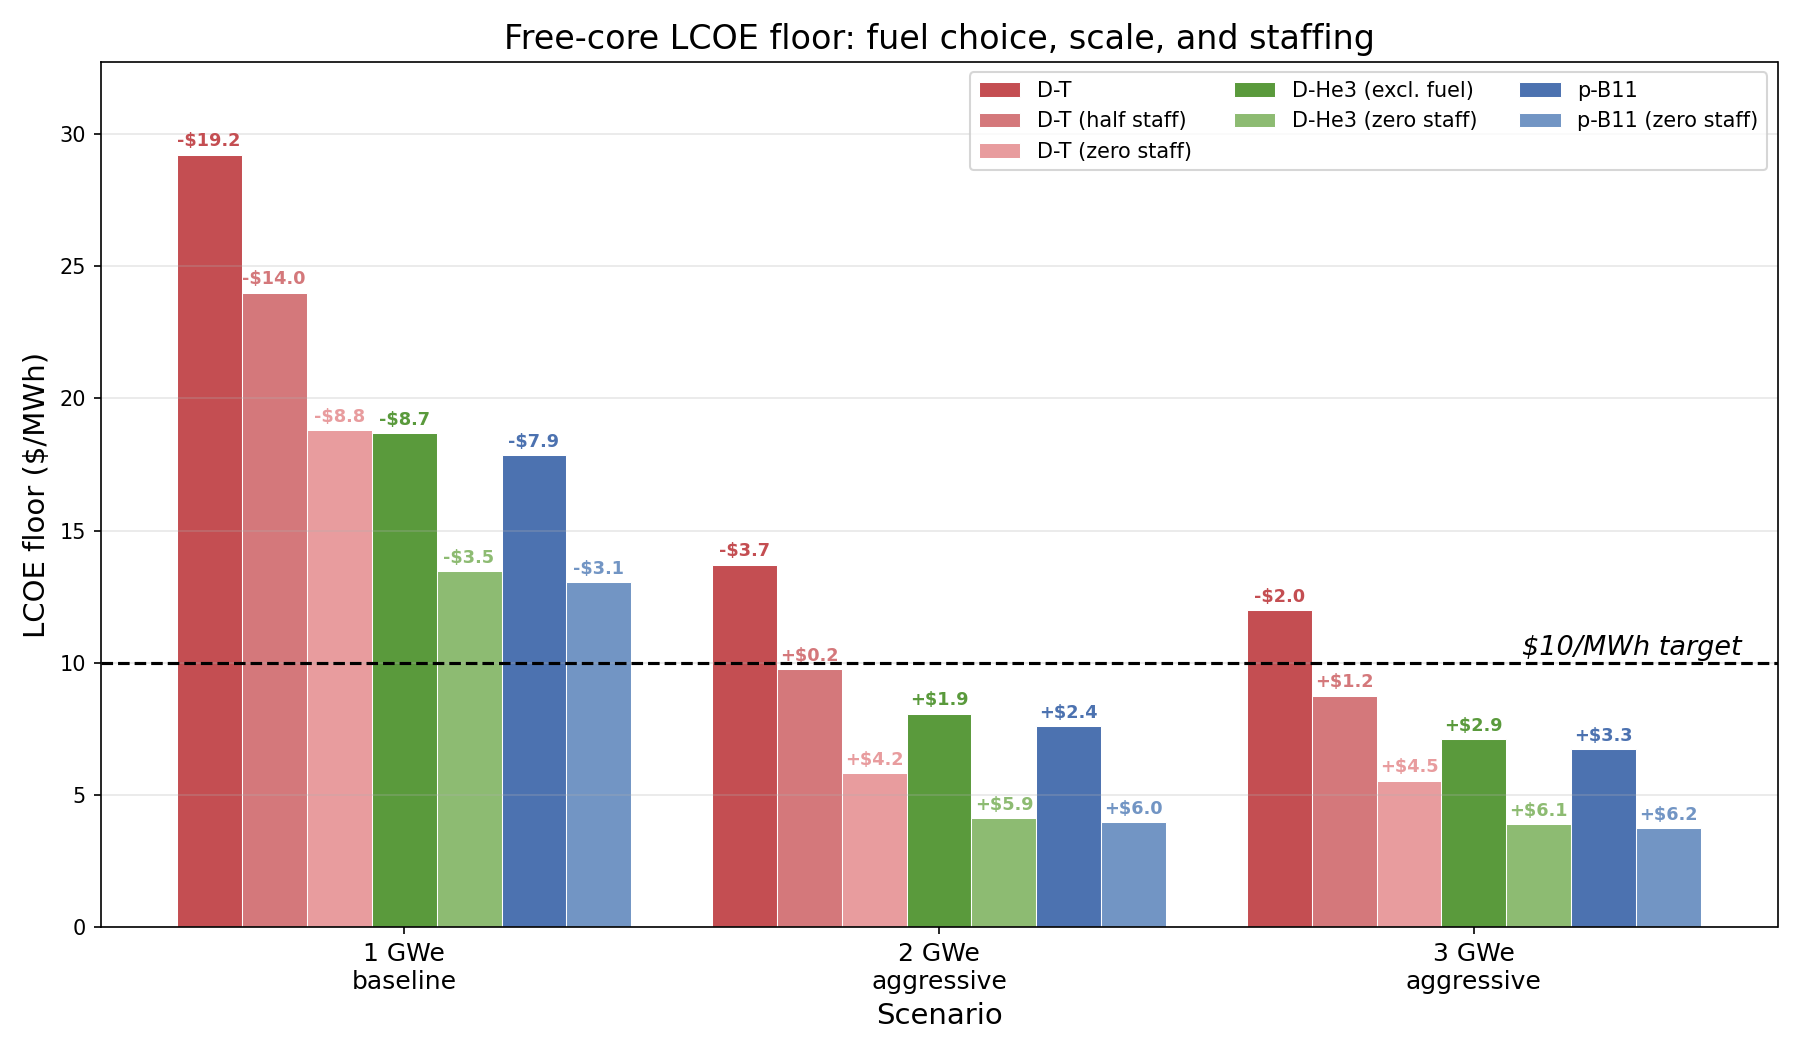
\includegraphics[width=0.85\linewidth]{figures/lower_bound_floor_chart.png}
\caption{Floor LCOE for D-T, D-He3, and p-B11 under three scenario
levels. Baseline assumes 1\,GWe, 85\% availability, 7\% WACC,
30-year lifetime, and 6-year construction. The aggressive scenario
(see Section~\ref{sec:dt}) is shown at 2\,GWe and at 3\,GWe.}
\label{fig:lower-bound}
\end{figure}

\subsection{Staffing and Automation}
\label{sec:staffing}

Operations and maintenance costs are dominated by staffing. At the
aggressive 5\,GWe D-T limit, O\&M contributes \$5.2/MWh of the
\$9.6/MWh floor; the capital-only component is \$4.3/MWh.
Halving D-T staffing from 78 to 39 FTE through SCADA-automated grid
dispatch, reduced shift coverage, and streamlined radiation
protection procedures (each realistic with current industrial
automation) lowers the 2\,GWe aggressive D-T floor to
\$10/MWh, although still leaving negligible budget for the costed
core. Lights-out operation, in the sense of a near-zero-FTE plant,
is constrained more by regulatory accountability than by technical
capability for the parameter ranges considered.

For p-B11, where no radiation-specific roles exist, automation
extends to a data-center-like operating model that strips both
staffing and the buildings supporting human occupancy. Together,
near-zero staffing and the associated building scope reduction
lower the 2\,GWe aggressive p-B11 floor from \$7.6/MWh to
approximately \$4.3/MWh, widening the available budget for the
costed core to \$5.7/MWh.

\subsection{Floor Findings}
\label{sec:floor-findings}

Four conclusions follow from this section.
\begin{itemize}
\item The D-T floor reaches the one-cent target only at extreme
scale with favorable financing, leaving negligible budget for the
costed core.
\item Fuel choice exerts a balance-of-plant lever larger than most
published core cost-reduction scenarios; aneutronic fuel downgrades
the buildings from enhanced-industrial to industrial and removes
tritium infrastructure entirely.
\item No single non-core parameter reaches the target; simultaneous
scale, availability, financing, and construction-time advantages
are required.
\item Plant scale provides more LCOE leverage than any other single
parameter, owing to the sublinear scaling of staffing with capacity.
\end{itemize}

The preceding analysis assumed a thermal energy conversion cycle.
For aneutronic fuels, this assumption is optional: the
charged-particle component of the fusion energy can in principle be
converted directly to electricity without intermediate heat
transfer. The remainder of this paper examines whether this
alternative architecture lowers the floor characterized in
Section~\ref{sec:floor}, and where its leverage lies if not.

\section{Direct Energy Conversion Architectures}
\label{sec:dec}

The energetic charged particles produced by fusion may be converted
directly to electricity without an intermediate heat-engine cycle.
The thermodynamic motivation is straightforward: charged particles
emerge from fusion plasmas at $10^8$--$10^9$\,K, so the Carnot
ceiling
\[
  \eta \leq 1 - T_\mathrm{cold}/T_\mathrm{hot}
\]
is essentially unity. This is a coarse upper bound: charged-particle
DEC of a thermal velocity distribution remains entropy-bounded below
unity, with real efficiency set by velocity-distribution
irreversibilities rather than by the thermodynamic limit alone.
The thermal default is bounded by first-wall and blanket material
limits (500--700\,$^\circ$C for RAFM steel and SiC composites),
which cap the Carnot limit near 60--65\% against a 300\,K cold sink.
Real thermal cycles lose 10--15 percentage points to heat-exchanger
and turbine irreversibilities, leaving sCO\textsubscript{2} Brayton
at 47\% and combined-cycle at 53\%. Charged-particle DEC has its
own irreversibilities, but the upper bound is higher.

\subsection{Fuel and Conversion Channels}
\label{sec:channels}

Charged-particle DEC operates only on charged particles. Neutrons
carry no charge, and bremsstrahlung photons at keV energies have no
demonstrated direct-conversion path; a proposed cascading-Auger
photovoltaic conversion of bremsstrahlung \citep{Binderbauer2018}
remains untested. DEC therefore favors fuel cycles with a small
neutron fraction.

The energy split among neutrons, charged particles, and
bremsstrahlung depends on fuel choice and operating point
(Figure~\ref{fig:channels}). For p-B11, the high plasma
temperature ($>$100\,keV) and Z=5 boron drive intense bremsstrahlung:
roughly 97\% of fusion power in a thermonuclear plasma, leaving a
3\% margin in the charged-particle channel \citep{Putvinski2019}.
Driving the plasma out of equilibrium widens the margin to
17\% \citep{Ochs2022}, but bremsstrahlung still
carries 83\% of the fusion power and deposits as heat on the walls.
Power flow for a thermal-only p-B11 mirror is summarized in
Figure~\ref{fig:pB11-thermal}.

\begin{figure}[htbp]
\centering
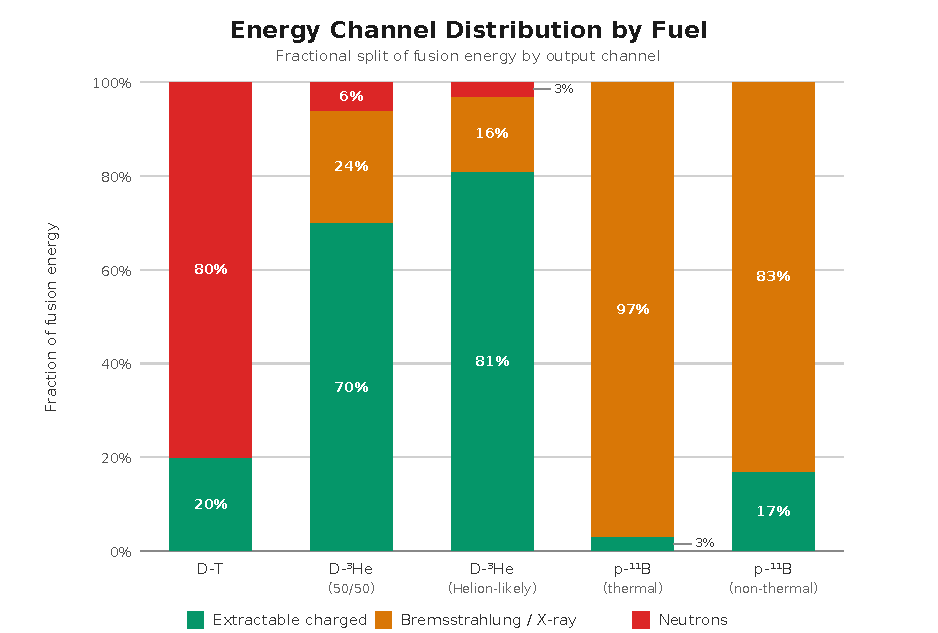
\includegraphics[width=0.7\linewidth]{figures/energy_channel_distribution.pdf}
\caption{Fractional split of fusion energy among neutrons, charged
particles, and bremsstrahlung as a function of fuel and operating
point. The deuterium-rich D-He3 plasmoid case maximizes the
charged-particle fraction.}
\label{fig:channels}
\end{figure}

\begin{figure}[htbp]
\centering
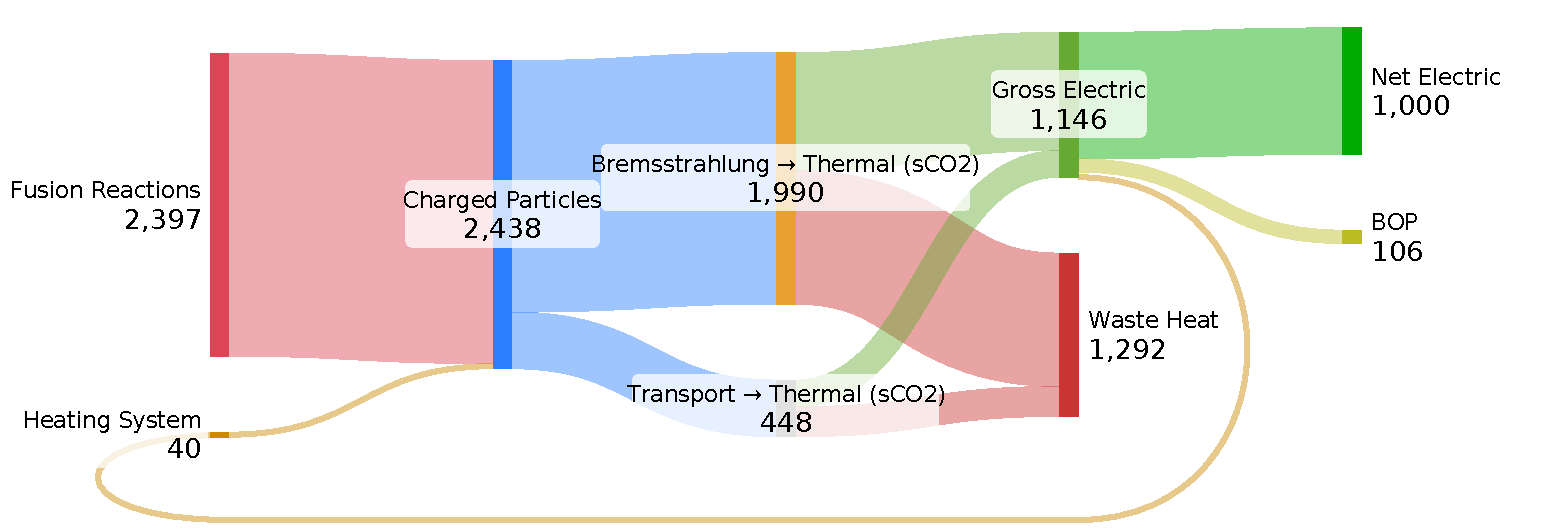
\includegraphics[width=0.85\linewidth]{figures/pB11_thermal_cycle.pdf}
\caption{Power flow in a 1\,GWe thermal-only p-B11 mirror: 83\% of
fusion power (1{,}990\,MW) is re-radiated as bremsstrahlung;
17\% (448\,MW) escapes as charged-particle transport; both feed a
single sCO\textsubscript{2} turbine at 47\%.}
\label{fig:pB11-thermal}
\end{figure}

D-He3 is the most favorable charged-particle DEC fuel. The primary
D-He3 reaction is aneutronic; D-D side reactions produce neutrons
and tritium, with the split depending on temperature, the
$n_D/n_{\mathrm{He3}}$ ratio, and confinement time. In a
steady-state plasma at 50/50 mix and $T = 70$\,keV, the bred
tritium fuses with deuterium and adds 14\,MeV neutrons
\citep{Wesson2004}. A
magneto-inertial plasmoid confines the plasma too briefly for the
secondary D-T reaction; the unburned tritium is exhausted, and the
14\,MeV neutron channel is eliminated. The mix can then be optimized
to minimize bremsstrahlung. A deuterium-rich operating point
($n_D/n_{\mathrm{He3}} = 3.2$ at $T = 100$\,keV) routes 81\% of
fusion energy into the charged-particle channel.

\subsection{The Bremsstrahlung Constraint}
\label{sec:brem}

The bremsstrahlung-dominated split established above forces every
charged-particle DEC architecture for p-B11 into the same
constraint.\footnote{Synchrotron emission does not impose a
comparable constraint. The fundamental electron cyclotron frequency
at 10\,T is 280\,GHz ($1.2 \times 10^{-3}$\,eV), with harmonics
extending into the THz band at fusion electron temperatures, six
orders of magnitude below bremsstrahlung. Mm-wave synchrotron
radiation reflects at $>$99\% from polished metallic first walls
and is typically recycled into the plasma. The escaping
few-percent fraction could in principle feed a rectenna using
mature GHz-band hardware, but the upside is bounded.} The thermal plant is not a small bottoming cycle in a
p-B11 plant; it is the primary conversion pathway, and DEC captures
only the charged-particle margin. Four options exist for the radiated fraction: (i) a full
thermal cycle converting bremsstrahlung heat at 47--53\%, retaining
essentially the full thermal BOP; (ii) magnetohydrodynamic (MHD)
conversion on a liquid-metal coolant, with theoretical efficiency
above 60\% but no fusion-scale demonstration \citep{Smolentsev2021};
(iii) rejection as waste heat, which collapses the overall plant
efficiency to roughly 14\% of fusion power as electricity (worse
than thermal-only at 47\%); and (iv) X-ray photovoltaic conversion
via cascading Auger emission in nanometric layered structures
\citep{Binderbauer2018}, currently a TRL\,1 concept. Of these, only
option (i) has a demonstrated path.

\subsection{Modeled Architectures}
\label{sec:modeled}

Two charged-particle DEC architectures are modeled: a venetian-blind
hybrid for p-B11 in a magnetic mirror, and an inductive scheme for
D-He3 in a compressed plasmoid. Both are evaluated against
thermal-cycle baselines. The cost basis for the thermal capture
hardware draws on a century of manufacturing cost-down and
well-understood n-th-of-a-kind pricing. The DEC cost estimates rest
on thinner ground: 1977 EPRI/LLNL studies for the venetian blind
\citep{Hoffman1977}, and a single capacitor build-up for the pulsed
inductive scheme; both are closer to first-of-a-kind than to the
turbines they would displace.

\subsubsection{Venetian-Blind Hybrid for p-B11}
\label{sec:vb}

The venetian-blind collector \citep{MoirBarr1973} consists of
angled metallic ribbon grids at successively higher retarding
potentials that sort ions by energy and collect them on
high-potential electrodes. It mounts on linear devices such as
magnetic mirrors as an add-on to the expander tank, capturing the
particle stream leaving along field lines. There are no moving
parts. The architecture was demonstrated at 48\% efficiency on real
end-loss plasma \citep{BarrMoir1983}, with a theoretical maximum of
70\% set by grid geometry and ion energy spread.

The p-B11 mirror baseline of Section~\ref{sec:floor} is carried
forward, and the venetian blind is added as an overlay. The thermal
cycle is retained for the bremsstrahlung-dominated channel
(Section~\ref{sec:channels}); the DEC captures only the charged
particles leaving the mirror axially, modeled at 90\% geometric
capture efficiency. The required fusion power is lower than the
thermal-only case (Figure~\ref{fig:pB11-thermal}) because the
venetian-blind hybrid contributes a fraction of net electric output
at higher conversion efficiency. The resulting power flow is shown
in Figure~\ref{fig:pB11-VB}. Sizing the venetian-blind hardware for
400\,MWe DEC output (n-th-of-a-kind, 2024 USD) yields approximately
\$125M total, in the range \$90--175M, comparable to the
partially-replaced turbine island (\$168M for sCO\textsubscript{2}
at 1\,GWe). The breakdown comprises high-voltage power
conditioning (\$45M), cryopumps (\$15M), thermal panels (\$15M),
grid and collector hardware (\$15M), high-voltage bushings, valves,
and controls (\$12M), a stainless-steel vacuum tank (\$7M), and
15\% installation. Power-conditioning costs are benchmarked against
contemporary VSC HVDC station pricing and ITER neutral-beam
injection components \citep{Hemsworth2017}; thermal panels follow
the design analog of the ITER NBI residual-ion dump and calorimeter;
grid and collector hardware use the geometric scaling of
\citet{Hoffman1977} escalated by CPI and cross-checked against
\citet{BarrMoir1983}.

\begin{figure}[htbp]
\centering
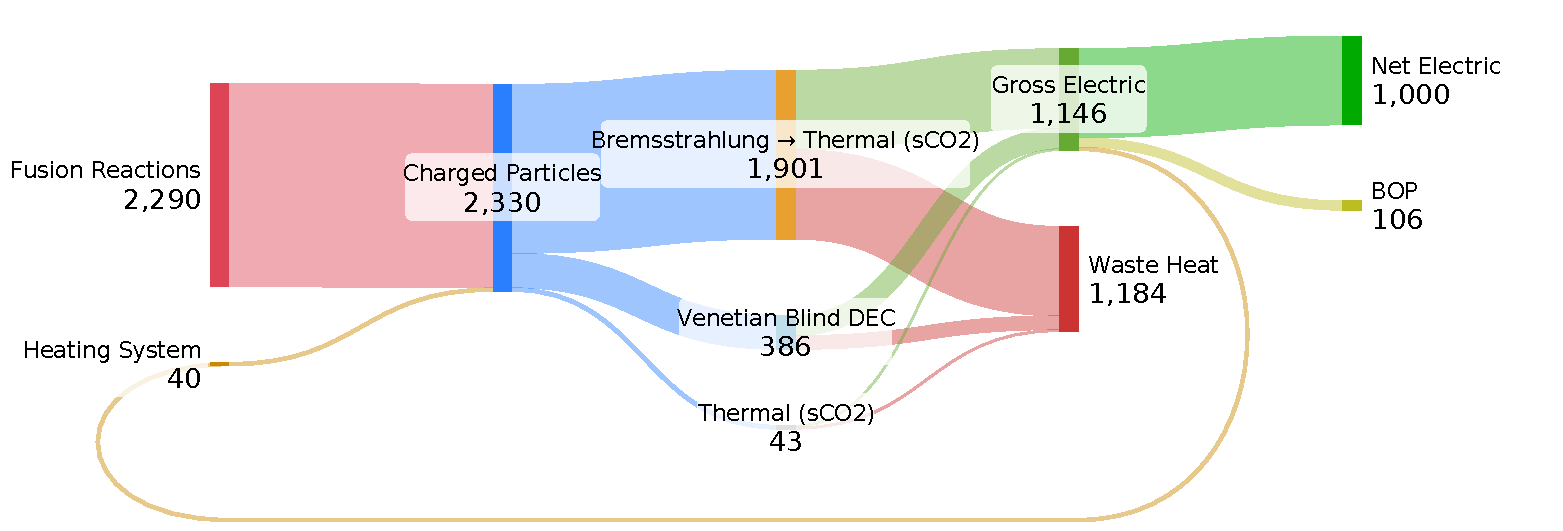
\includegraphics[width=0.85\linewidth]{figures/pB11_VB_DEC.pdf}
\caption{Power flow in a 1\,GWe p-B11 mirror with a venetian-blind
DEC at 60\% in hybrid configuration with a thermal cycle: 83\% of
fusion power (1{,}901\,MW) feeds the turbine; the DEC captures
90\% of the 17\% charged-particle margin (386\,MW).}
\label{fig:pB11-VB}
\end{figure}

\begin{table}[htbp]
\caption{p-B11 mirror configurations at 1\,GWe with a free fusion
core.}
\label{tab:vb}
\centering
\begin{tabular}{lrr}
\toprule
Configuration & Floor (\$/MWh) & Overnight (\$/kW) \\
\midrule
Thermal only (sCO\textsubscript{2} Brayton, 47\%) & 18 & 1{,}221 \\
VB DEC at 48\% + thermal (hybrid) & 19 & 1{,}253 \\
VB DEC at 60\% + thermal (hybrid) & 19 & 1{,}246 \\
\bottomrule
\end{tabular}
\end{table}

The venetian blind does not lower the floor (Table~\ref{tab:vb}).
With 83\% of fusion energy in bremsstrahlung, the DEC captures 90\%
of the 17\% charged-particle margin. At the demonstrated 48\%
efficiency the DEC hardware adds cost without meaningful improvement
in conversion. Even at 60\% (never demonstrated on real plasma),
the hybrid floor is \$19/MWh, \$1/MWh above thermal-only, with
\$25--30/kW additional overnight capital. Eliminating
the turbine entirely and rejecting the bremsstrahlung is not viable
for p-B11: a non-thermal plant requires roughly 11\,GW of fusion
power for 1\,GWe net (net efficiency: 17\% charged-particle margin
times 60\% DEC efficiency times 90\% geometric capture), so the
required fusion power exceeds the thermal path's by a factor of
roughly five.

A break-even analysis, holding venetian-blind hardware cost fixed at
the 1\,GWe baseline value of \$85M, finds no efficiency in the
30--100\% range that justifies adding the DEC against thermal-only.
The DEC hardware cost exceeds the turbine-side savings across the
entire physically accessible band. Break-even enters the accessible
window only if the venetian-blind capital expenditure at this plant
scale falls by approximately a factor of three (to \$30M), at
which point a 54\% efficiency suffices.

\subsubsection{Pulsed Inductive DEC for D-He3}
\label{sec:pulsed}

Pulsed inductive DEC employs coils surrounding a compression chamber
that compress a pulsed plasmoid and then recover energy as the
plasmoid re-expands, inducing current via Faraday's law and
requiring no plasma-surface contact \citep{Slough2011}. The same
coils drive both halves of the cycle. No published demonstration on
fusion plasma exists. At the deuterium-rich operating point
($n_D/n_{\mathrm{He3}} = 3.2$, $T = 100$\,keV, no tritium burnup),
81\% of fusion energy enters the charged-particle channel and
drives the inductive coils. Unlike the venetian-blind hybrid, no
main turbine is retained and no thermal bottoming cycle is added;
the pulsed-power chain is the only conversion stage, and the
bremsstrahlung and neutron fractions are dumped to cooling as waste
heat. The resulting power flow is shown in
Figure~\ref{fig:DHe3-pulsed}.

\begin{figure}[htbp]
\centering
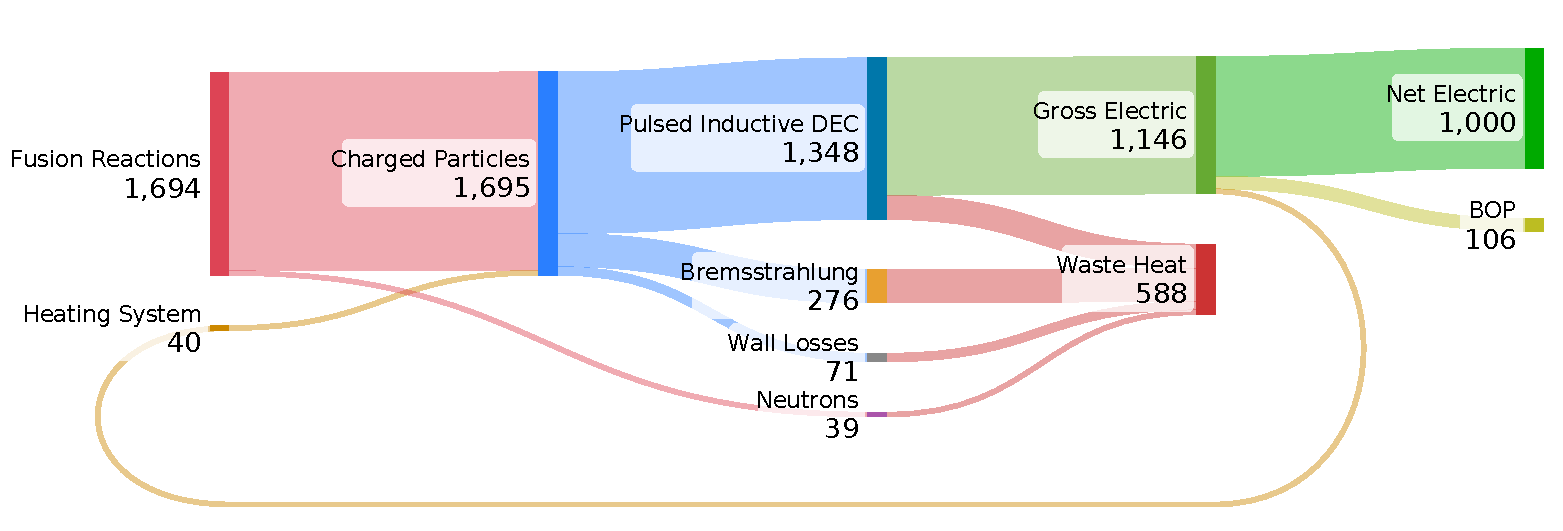
\includegraphics[width=0.85\linewidth]{figures/DHe3_pulsed_inductive.pdf}
\caption{Power flow in a 1\,GWe D-He3 plant at the deuterium-rich
operating point ($n_D/n_{\mathrm{He3}} = 3.2$, $T = 100$\,keV,
tritium exhausted, 99\% inter-shot helium-3 recovery, no thermal
bottoming): 1{,}348\,MW of charged-particle transport drives the
pulsed inductive DEC at 85\%; bremsstrahlung (276\,MW), neutrons
(39\,MW), and DEC waste are dumped to cooling. Total fusion power
$P_\mathrm{fus} = 1{,}695$\,MW.}
\label{fig:DHe3-pulsed}
\end{figure}

The pulsed-power chain comprises pulse-rated switchgear, capacitor
or inductive storage to smooth the duty cycle, DC-DC converters to
recharge the compression coils, and a grid-tie inverter at the
output. Sizing the chain downstream of the driver to 1\,GWe net
(n-th-of-a-kind) yields \$593M (\$593/kW total),
distributed as recovery capacitor bank (\$351M, 703\,MJ at
\$0.50/J), VSC HVDC valve hall and IGBT grid-tie (\$150M,
\$150/kW net), DC-DC links (\$78M, \$75/kW gross), and controls
(\$14M, 4\% of the driver bank). The \$593M total reported in
Table~\ref{tab:pulsed} excludes the compression capacitor bank,
which is treated as part of the costed core in the model and is
not part of the BOP floor.

\begin{table}[htbp]
\caption{D-He3 plant configurations at 1\,GWe with a free fusion
core. Helium-3 fuel cost assumed \$2M/kg.}
\label{tab:pulsed}
\centering
\begin{tabular}{lrrr}
\toprule
Configuration & BOP floor (\$/MWh) & He-3 fuel (\$/MWh) & Total
(\$/MWh) \\
\midrule
Thermal only (sCO\textsubscript{2} Brayton, 47\%) & 19 & 74 & 93 \\
Pulsed inductive (85\% $\eta$, no turbine) & 24 & 36 & 59 \\
\bottomrule
\end{tabular}
\end{table}

The BOP floor is \$6/MWh higher than the thermal baseline
(Table~\ref{tab:pulsed}). The turbine island is not the dominant
cost in the thermal plant; buildings (\$354M), the electrical
plant (\$96M), the operations and maintenance budget
(\$37M per year), and financing charges together exceed it.
Eliminating the turbine and synchronous generator removes
\$186M of overnight capital, but the \$593M
pulsed-power chain that replaces it more than offsets the savings.

The fuel cost is a separate concern. At \$2M/kg, helium-3
contributes \$36/MWh to LCOE for the inductive architecture; at
the DOE-allocated price of \$4.5M/kg, this doubles.
The deuterium-rich operating mix maximizes D-D-bred helium-3 and
recovers it between shots at an assumed 99\% efficiency, lowering
external helium-3 demand by approximately a quarter relative to the
50/50 reference. Mix selection saves \$20/MWh of LCOE,
almost entirely through reduced helium-3 burn. Even if external
fuel cost is driven to zero (self-bred), the BOP floor remains
\$24/MWh, still above the thermal baseline (\$18/MWh) and above
the one-cent target.

The plasma-present round-trip efficiency is the primary open
parameter. The theoretical framework of \citet{Kirtley2024}
suggests 85\% as a realistic target. At that level, the reduction
of required fusion power by one-third and external
helium-3 burn by more than half drives the economic case for the
architecture, not the BOP hardware (which already costs more than
a turbine).

The role of round-trip efficiency in this architecture differs from
that of efficiency in a thermal cycle. With no thermal-only
fallback, the inductive recovery stage is intrinsic: efficiency
below the round-trip threshold yields no net electric output,
making efficiency a gating condition for breakeven rather than a
cost knob. Above the threshold, the plant operates with high
recirculating power by construction, and LCOE tracks the small net
output rather than the large gross. Enabling and economic
viability are therefore distinct thresholds; clearing the first
does not imply clearing the second.

\subsection{The Industrial Floor Persists}
\label{sec:converge}

The aggressive scenario collapses the gap between thermal and DEC
for both fuels (Table~\ref{tab:agg}). For p-B11, the hybrid DEC and thermal-only
configurations land within \$0.2/MWh; the DEC overlay costs
as much as the thermal hardware it partially replaces. Pulsed inductive is not viable for p-B11 because
rejecting 83\% of fusion energy as bremsstrahlung requires a much
larger core. For D-He3, helium-3 fuel at \$2M/kg dominates
everything else; self-breeding closes the fuel gap, and the
inductive scheme then ends up \$6/MWh higher than thermal because
the pulsed-power chain is more expensive than the turbine.

\begin{table}[htbp]
\caption{Conversion architectures under the aggressive scenario
(see Section~\ref{sec:dt}).}
\label{tab:agg}
\centering
\begin{tabular}{lrrr}
\toprule
Approach & p-B11 & D-He3 (\$2M/kg) & D-He3 (self-bred) \\
\midrule
Thermal only (sCO\textsubscript{2}, 47\%) & 7.6 & 82\footnote{Aggressive
financing reduces the BOP-floor contribution; the helium-3 fuel
cost at \$2M/kg is independent of plant financing.} & 8 \\
VB DEC 60\% + thermal (hybrid) & 7.9 & 82 & 9 \\
Pulsed inductive (85\%, no turbine) & n/a & 55 & 14 \\
\bottomrule
\end{tabular}
\end{table}

The floor is set by the industrial cost of building, staffing, and
financing a large power plant, not by the choice of power
conversion architecture. The leverage of DEC, where it exists, is
exerted on the costed core or on the fuel bill rather than on the
floor.

\subsection{Where DEC Exerts Leverage}
\label{sec:where}

In the fully costed plant, DEC's value emerges through two
mechanisms: a higher conversion efficiency reduces the fusion power
required for a given net electric output, lowering the costed-core
capital; and for expensive fuels, the lower fusion power also
reduces the fuel bill. The two fuel cycles respond differently.

For D-He3 at 1\,GWe baseline, the venetian-blind hybrid lowers
LCOE from \$114/MWh to \$104/MWh, with a modest \$23M
increase in core cost partially offset by reduced heating-system
capacity. The pulsed inductive scheme lowers LCOE to \$76/MWh,
with the savings driven primarily by fuel rather than by hardware:
higher conversion efficiency, the deuterium-rich operating mix, and
inter-shot helium-3 recovery together reduce external helium-3
demand. For D-He3, DEC is therefore predominantly a fuel-saving
technology.

For p-B11 (negligible fuel cost), the second channel disappears
and only the core-shrinkage channel remains. Because bremsstrahlung
dominates the energy split, even an efficient DEC captures only the
17\% charged-particle margin and does not meaningfully reduce the
required fusion power. Thermal LCOE is \$37/MWh; the
venetian-blind DEC at 60\% yields \$37/MWh as well, with core
costs of \$1{,}202M and \$1{,}234M respectively. The DEC overlay
neither lowers the floor nor shrinks the core enough to pay for
itself.

\subsection{Learning Rates}
\label{sec:learning}

The numbers above represent snapshots; deployed technologies become
cheaper. Steam and gas turbines have been manufactured for over a
century with thousands of GW deployed, and little learning headroom
remains. The DEC architectures sit at lower technology readiness
levels with larger cost uncertainties and more headroom.

The venetian blind is the most mature DEC option (TRL 4--5 on
non-fusion plasma). Its dominant cost components (vacuum vessels,
cryopumps) are mature industrial hardware contributing 75\% of
total cost; the grids contribute 2\%. The cost-down
opportunity is therefore limited.

The pulsed inductive path differs. Capacitor banks and power
electronics dominate, and both are early in their deployment
curves. The n-th-of-a-kind assumption used here is \$0.50/J of
energy stored (all-in: capacitors, switches, charging, busswork)
drawn from the extension to the fusion costing standard
\citep{CATF2026}. Contemporary laboratory pricing is \$20--50/J,
a 40--100$\times$ gap, comparable in magnitude to the cost-down
achieved by solar photovoltaics over two decades
\citep{Ramasamy2025}. Grid-tie inverters have already followed a
similar curve (from \$1{,}000/kW in the early 2000s to
\$100--150/kW today). The fusion-specific components (capacitors
rated for $10^8$ cycles at high energy density) do not yet exist
as commercial products; the \$0.50/J figure is a target rather
than a current price. Should capacitor pricing remain at
\$5--20/J, the pulsed floors would increase substantially and the
economic balance would favor a turbine. Capacitor lifetime
compounds the risk: current high-energy-density capacitors achieve
$10^7$ cycles, which at 1\,Hz repetition corresponds to
four months of operation between bank replacements. The thermal
and venetian-blind floors carry no comparable risk. The efficiency
and cost ranges for the four conversion paths are summarized in
Figure~\ref{fig:efficiency-cost}.

\begin{figure}[htbp]
\centering
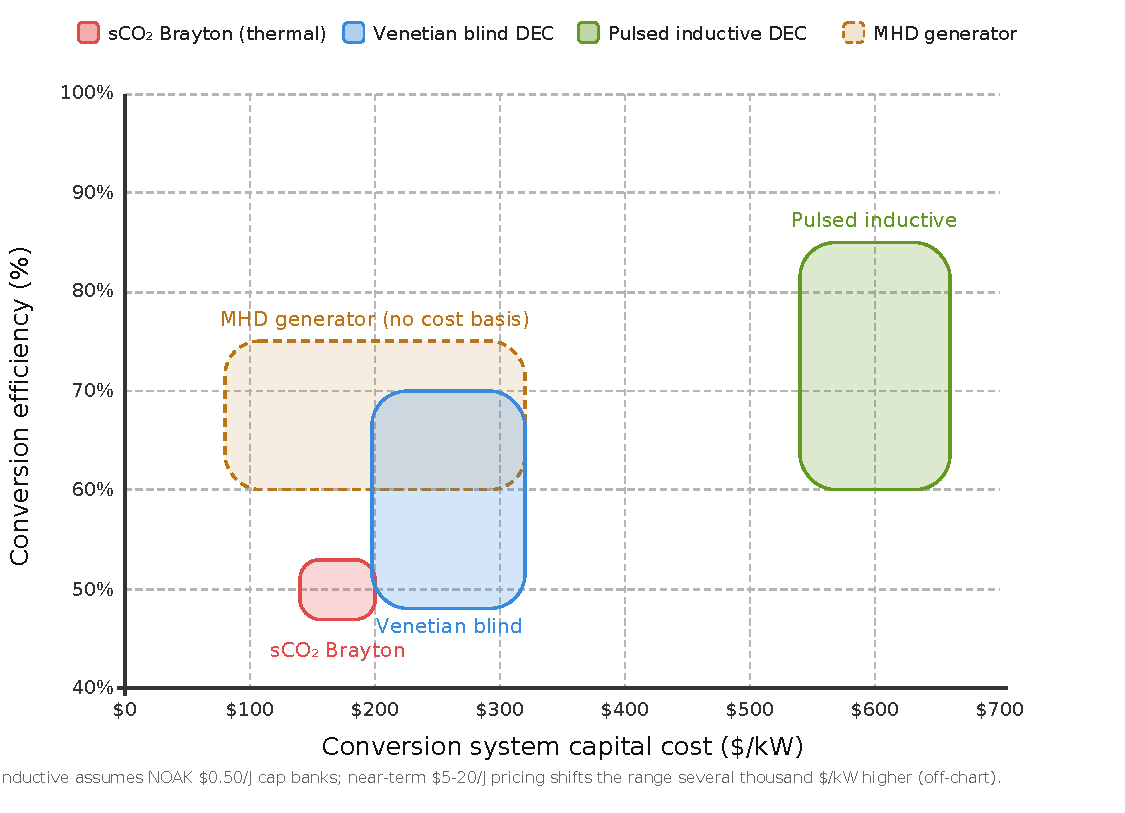
\includegraphics[width=0.85\linewidth]{figures/efficiency_cost_chart.pdf}
\caption{Conversion efficiency (vertical axis) and overnight
capital cost in dollars per kilowatt (horizontal axis) for the four
conversion architectures: sCO\textsubscript{2} Brayton,
venetian-blind DEC plus thermal hybrid, pulsed inductive DEC, and
(dashed) liquid-metal MHD. The MHD entry is shown dashed because no
fusion-relevant cost basis exists; the pulsed inductive entry
assumes the \$0.50/J n-th-of-a-kind capacitor target.}
\label{fig:efficiency-cost}
\end{figure}

\section{Discussion}
\label{sec:discuss}

The cost of fusion electricity is set primarily by the industrial
fabric around the core (buildings, balance-of-plant, staffing, and
financing). The leverage of DEC is exerted on the costed core and
on the fuel bill rather than on the floor: for p-B11,
bremsstrahlung dominates the energy split and the venetian-blind
hybrid neither lowers nor meaningfully increases the floor relative
to thermal-only; for D-He3, the inductive scheme reduces the fusion
power and helium-3 burn rate but substitutes a pulsed-power chain
that costs more than a turbine. Three experimental milestones would
convert this opportunity into evidence.

\section{Future Directions}
\label{sec:future}

Three experimentally tractable targets are identified.
\begin{itemize}
\item Sustained venetian-blind efficiency above 60\% on real plasma.
\item Pulsed inductive round-trip efficiency above 85\% on a
representative plasmoid device.
\item Demonstration of MHD liquid-metal generators at
fusion-relevant magnetic field strengths
\citep{Smolentsev2021}.
\end{itemize}
Each is an experimental program rather than a research miracle.
The path to one-cent fusion energy does not run through DEC alone,
but DEC retains cost-down headroom in directions the thermal path
lacks.

\section*{Acknowledgements}
The authors thank Mallory Snowden, Ian Ochs, Elijah Kolmes, and
Ryan Weed for useful discussions.

\bibliographystyle{unsrtnat}
\bibliography{references}

\end{document}
